
\subsection{Meta-transfer learning (MTL)}
\label{sec_meta_transfer}

As shown in Figure~\ref{main_framework_meta_transf_hard_task}(b), our proposed meta-transfer learning (MTL) method optimizes the meta operations \emph{Scaling} and \emph{Shifting} (\emph{SS}) through HT meta-batch training (Section~\ref{sec_HT}). 
%
Figure~\ref{main_framework_SS_FT} visualizes the difference of updating through \emph{SS} and \emph{FT}.
\emph{SS} operations, denoted as $\Phi_{S_1}$ and $\Phi_{S_2}$, do not change the frozen neuron weights of $\Theta$ during learning, while \emph{FT} updates the complete $\Theta$. 
%

In the following, we detail the \emph{SS} operations.
%
%
Given a task $\mathcal{T}$, the loss of $\mathcal{T}^{(tr)}$ is used to optimize the current base-learner (classifier) $\theta'$ by gradient descent:
\begin{equation}\label{eq_base_classifier}
  \theta' \gets \theta - \beta\nabla_{\theta}\mathcal{L}_{\mathcal{T}^{(tr)}}\big([\Theta; \theta], \Phi_{S_{\{1,2\}}}\big),
\end{equation}
which is different to Eq.~\ref{eq_large_scale_update}, as we do not update $\Theta$. 
Note that here $\theta$ is different to the one from the previous phase, the large-scale classifier $\theta$ in Eq.~\ref{eq_large_scale_update}. 
%
This $\theta$ concerns only a few of classes, e.g. 5 classes, to classify each time in a novel few-shot setting. 
%
$\theta'$ corresponds to a temporal classifier only working in the current task, initialized by the $\theta$ optimized for the previous task (see Eq.~\ref{eq_meta_classifier}). 


$\Phi_{S_1}$ is initialized by ones and $\Phi_{S_1}$ by zeros. Then, they are optimized by the test loss of $\mathcal{T}^{(te)}$ as follows,
%
\begin{equation}\label{eq_ss_update}
     \Phi_{S_i} =: \Phi_{S_i} - \gamma\nabla_{\Phi_{S_i}}\mathcal{L}_{\mathcal{T}^{(te)}}\big([\Theta; \theta'], \Phi_{S_{\{1,2\}}}\big).
\end{equation}
%
%
In this step, $\theta$ is updated with the same learning rate $\gamma$ as in Eq.~\ref{eq_ss_update},
\begin{equation}\label{eq_meta_classifier}
  \theta =: \theta - \gamma\nabla_{\theta}\mathcal{L}_{\mathcal{T}^{(te)}}\big([\Theta; \theta'], \Phi_{S_{\{1,2\}}}\big).
\end{equation}
Re-linking to Eq.~\ref{eq_base_classifier}, we note that the above $\theta'$ comes from the last epoch of base-learning on $\mathcal{T}^{(tr)}$.

Next, we describe how we apply $\Phi_{S_{\{1,2\}}}$ to the frozen neurons as shown in Figure~\ref{main_framework_SS_FT}(b). 
Given the trained $\Theta$, for its $l$-th layer containing $K$ neurons, we have $K$ pairs of parameters, respectively as weight and bias, denoted as $\{(W_{i,k}, b_{i,k})\}$. Note that the neuron location $l, k$ will be omitted for readability.
%
Based on MTL, we learn $K$ pairs of scalars $\{\Phi_{S_{\{1,2\}}}\}$. 
%
Assuming $X$ is input, we apply $\{\Phi_{S_{\{1,2\}}}\}$ to $(W, b)$ as
\begin{equation}\label{eq_SS_operation}
    SS(X; W, b; \Phi_{S_{\{1,2\}}}) =(W\odot\Phi_{S_1}) X + (b + \Phi_{S_2}),
\end{equation}
where $\odot$ denotes the element-wise multiplication.

\begin{figure}[t]
  \centering
  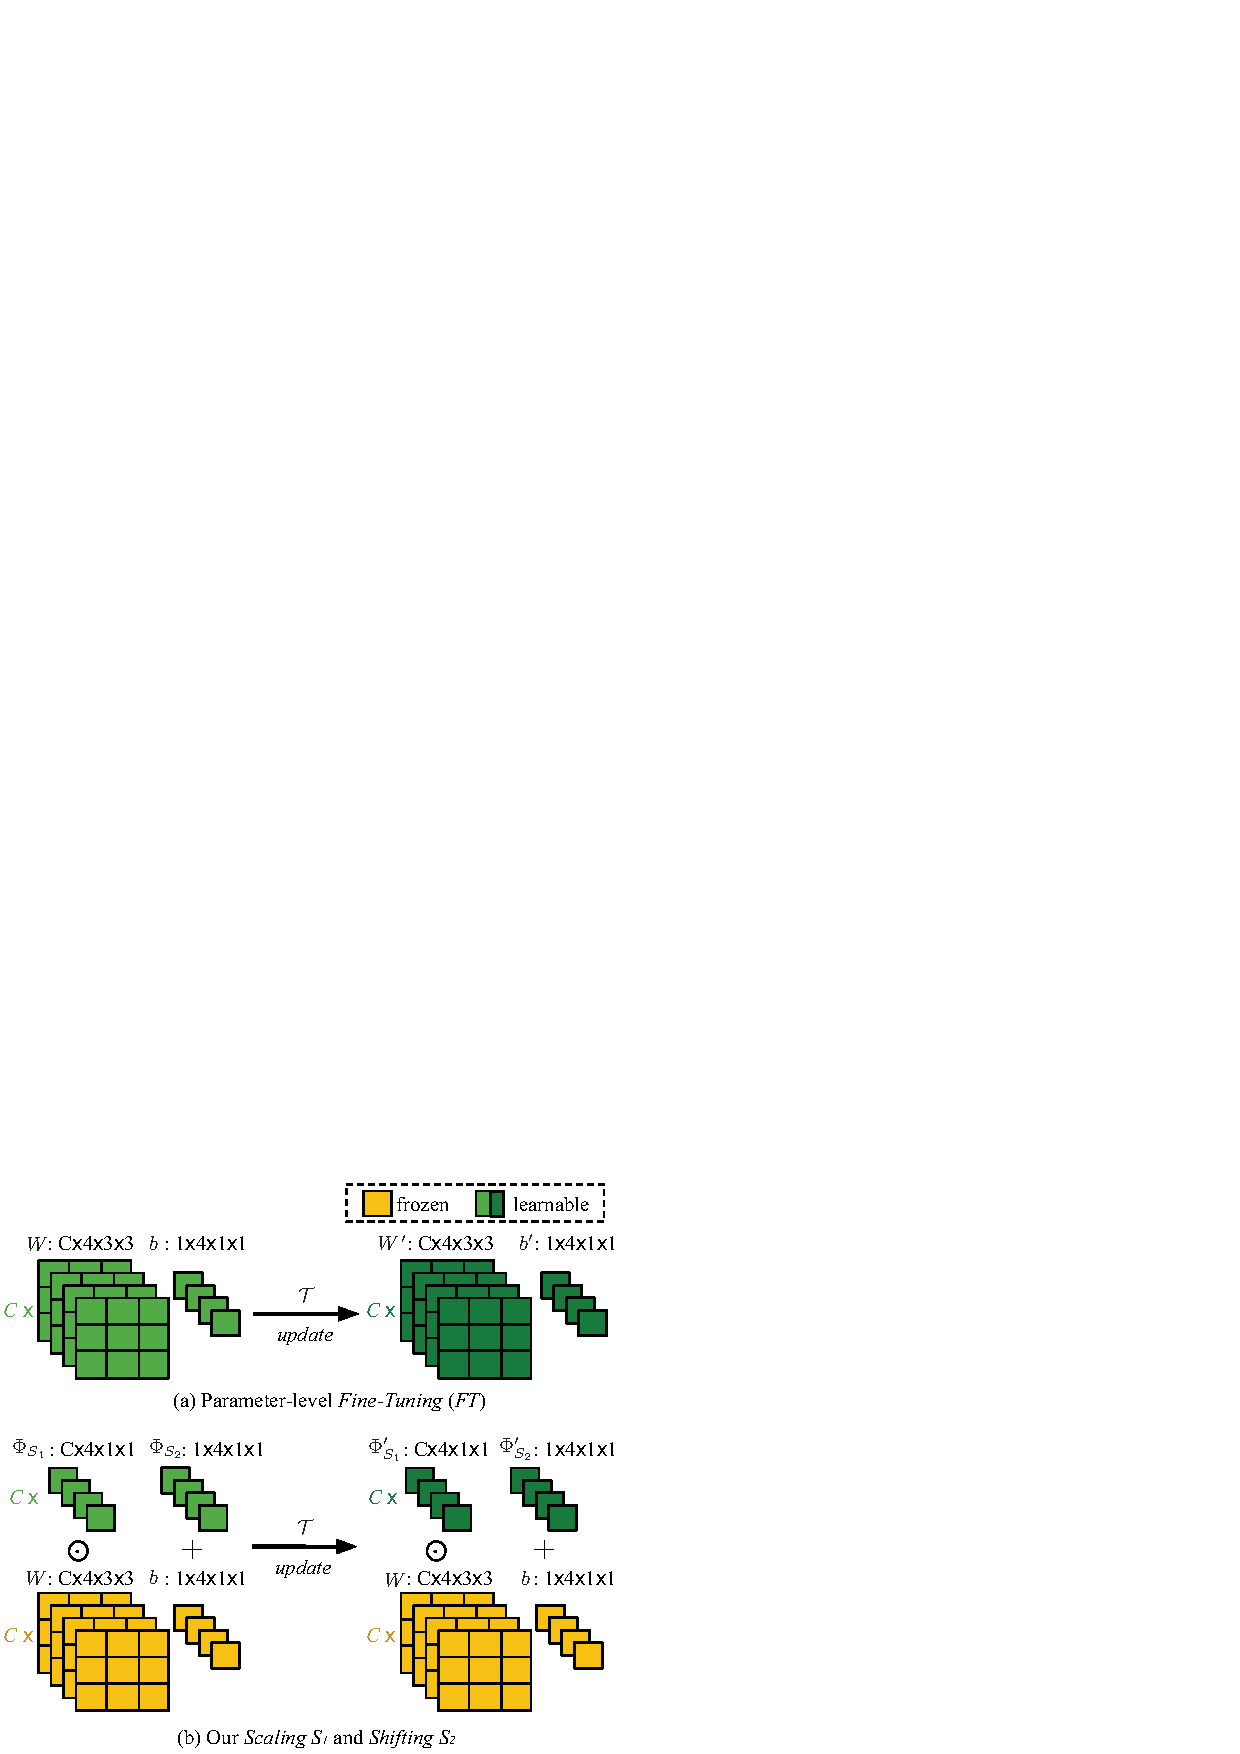
\includegraphics[width=0.99\linewidth]{figures/main_framework_SS_FT.pdf}
     \caption{(a) Parameter-level \emph{Fine-Tuning} (\emph{FT}) is a conventional meta-training operation, e.g. in MAML~\cite{FinnAL17}. Its update works for all neuron parameters, $W$ and $b$.
     (b) Our neuron-level \emph{Scaling} and \emph{Shifting} (\emph{SS}) operations in MTL. They reduce the number of learning parameters and avoid overfitting problems. In addition, they keep large-scale trained parameters (in yellow) frozen, preventing ``catastrophic fogetting''~\cite{LopezPazNIPS17, McCloskey1989}.
    }
  \label{main_framework_SS_FT}
\end{figure}


Taking Figure~\ref{main_framework_SS_FT}(b) as an example of a single $3\times 3$ filter, after \emph{SS} operations, this filter is scaled by $\Phi_{S_1}$ then the feature maps after convolutions are shifted by $\Phi_{S_2}$ in addition to the original bias $b$. 
Detailed steps of \emph{SS} are given in Algorithm~\ref{alg_Meta} in Section~\ref{sec_alg}.
%

Figure~\ref{main_framework_SS_FT}(a) shows a typical parameter-level \emph{Fine-Tuning} (\emph{FT}) operation, which is in the meta optimization phase of our related work MAML~\cite{FinnAL17}.
%
It is obvious that \emph{FT} updates the complete values of $W$ and $b$, and has a large number of parameters, and our \emph{SS} reduces this number to below $\tfrac{2}{9}$ in the example of the figure. 
%


In summary, \emph{SS} can benefit MTL in three aspects.
1) It starts from a strong initialization  based on a large-scale trained DNN, yielding fast convergence for MTL.
2) It does not change DNN weights, thereby avoiding the problem of ``catastrophic forgetting''~\cite{LopezPazNIPS17, McCloskey1989} when learning specific tasks in MTL.
3) It is light-weight, reducing the chance of overfitting of MTL in few-shot scenarios.
%
%



\subsection{Hard task (HT) meta-batch}
\label{sec_HT}

In this section, we introduce a method to schedule hard tasks in meta-training batches. 
%
The conventional meta-batch is composed of randomly sampled tasks, where the randomness implies random difficulties~\cite{FinnAL17}.
In our meta-training pipeline, we intentionally pick up failure cases in each task and re-compose their data to be harder tasks for adverse re-training. 
We aim to force our meta-learner to ``grow up through hardness''. 

\myparagraph{Pipeline.}
Each task $\mathcal{T}$ has two splits, $\mathcal{T}^{(tr)}$ and $\mathcal{T}^{(te)}$, for base-learning and test, respectively.
As shown in Algorithm~\ref{alg_Meta} line 2-5, base-learner is optimized by the loss of $\mathcal{T}^{(tr)}$ (in multiple epochs). \emph{SS} parameters are then optimized by the loss of $\mathcal{T}^{(te)}$ once.
%
We can also get the recognition accuracy of $\mathcal{T}^{(te)}$ for $M$ classes. Then, we choose the lowest accuracy $Acc_m$ to determine the most difficult class-$m$ (also called failure class) in the current task.

%
%
After obtaining all failure classes (indexed by $\{m\}$) from $k$ tasks in current meta-batch $\{\mathcal{T}_{1\sim k}\}$, we re-sample tasks from their data. 
%
Specifically, we assume $p(\mathcal{T}|\{m\})$ is the task distribution, we sample a ``harder'' task $\mathcal{T}^{hard} \in p(\mathcal{T}|\{m\})$.
Two important details are given below.


%
\myparagraph{Choosing hard class-$m$.} We choose the failure class-$m$ from each task by ranking the class-level accuracies instead of fixing a threshold.
%
In a dynamic online setting as ours, it is more sensible to choose the hardest cases based on ranking rather than fixing a threshold ahead of time. 
%

\myparagraph{Two methods of hard tasking using $\{m\}$.}
%
Chosen $\{m\}$, we can re-sample tasks $\mathcal{T}^{hard}$ by (1) directly using the samples of class-$m$ in the current task $\mathcal{T}$, or (2) indirectly using the label of class-$m$ to sample new samples of that class.
In fact, setting (2) considers to include more data variance of class-$m$ and it works better than setting (1) in general. 
%%


